% ============================================================
% 讲义 — 人教版九年级下册 · 第27章 相似
% 编译命令：xelatex -interaction=nonstopmode 第27章_相似.tex
% ============================================================
\documentclass[12pt, a4paper]{ctexart}
\usepackage[margin=2.2cm]{geometry}
\usepackage{amsmath, amssymb}
\usepackage{enumitem}
\usepackage{tcolorbox}
\usepackage{booktabs}
\usepackage{array}
\usepackage{fancyhdr}
\usepackage{xcolor}
\usepackage{tikz}
\usetikzlibrary{calc}
\usepackage{hyperref}
\usepackage{graphicx}
\usepackage{multirow}
\usepackage{pgfplots}
\pgfplotsset{compat=1.18}

% 颜色定义
\definecolor{mainblue}{RGB}{41, 98, 168}
\definecolor{lightblue}{RGB}{230, 240, 255}
\definecolor{tipgreen}{RGB}{34, 139, 87}
\definecolor{lightgreen}{RGB}{235, 250, 240}
\definecolor{warnred}{RGB}{200, 50, 50}
\definecolor{lightred}{RGB}{255, 240, 240}
\definecolor{examorange}{RGB}{210, 120, 20}
\definecolor{lightorange}{RGB}{255, 248, 235}
\definecolor{apppurple}{RGB}{120, 60, 170}
\definecolor{lightpurple}{RGB}{245, 238, 255}

% 页眉页脚
\pagestyle{fancy}
\fancyhf{}
\fancyhead[L]{\small\textcolor{mainblue}{\textbf{人教版九年级下册}}}
\fancyhead[R]{\small\textcolor{mainblue}{第27章 相似讲义}}
\fancyfoot[C]{\small —\ \thepage\ —}
\renewcommand{\headrulewidth}{0.6pt}
\renewcommand{\headrule}{\hbox to\headwidth{\color{mainblue}\leaders\hrule height \headrulewidth\hfill}}
\renewcommand{\footrulewidth}{0pt}

% tcolorbox 样式
\newtcolorbox{knowledgebox}[1][]{%
  colback=lightblue, colframe=mainblue,
  fonttitle=\bfseries\large, title=#1,
  arc=3mm, boxrule=0.8pt,
  left=8pt, right=8pt, top=6pt, bottom=6pt
}

\newtcolorbox{tipbox}[1][]{%
  colback=lightgreen, colframe=tipgreen,
  fonttitle=\bfseries, title=#1,
  arc=2mm, boxrule=0.6pt,
  left=6pt, right=6pt, top=4pt, bottom=4pt
}

\newtcolorbox{warnbox}[1][]{%
  colback=lightred, colframe=warnred,
  fonttitle=\bfseries, title=#1,
  arc=2mm, boxrule=0.6pt,
  left=6pt, right=6pt, top=4pt, bottom=4pt
}

\newtcolorbox{examplebox}[1][]{%
  colback=lightorange, colframe=examorange,
  fonttitle=\bfseries, title=#1,
  arc=3mm, boxrule=0.8pt,
  left=8pt, right=8pt, top=6pt, bottom=6pt
}

\newtcolorbox{appbox}[1][]{%
  colback=lightpurple, colframe=apppurple,
  fonttitle=\bfseries, title=#1,
  arc=3mm, boxrule=0.8pt,
  left=8pt, right=8pt, top=6pt, bottom=6pt
}

\setCJKmainfont{Hiragino Sans GB}
\setCJKsansfont{Heiti SC}

\begin{document}

% ============ 标题页 ============
\begin{center}
{\Huge\bfseries\textcolor{mainblue}{第27章\quad 相似}}\\[12pt]
{\Large\textcolor{gray}{讲\quad 义}}\\[8pt]
\rule{0.6\textwidth}{1pt}\\[8pt]
{\normalsize 适用：人教版\quad 九年级下册\quad |\quad 课时：8课时}
\end{center}
\vspace{10pt}

% ============================================================
%  第一部分：知识点讲解
% ============================================================
\section*{\textcolor{mainblue}{一、知识点讲解}}

% ------- 27.1 比例的基本性质 -------
\subsection*{27.1\quad 比例的基本性质}

\begin{knowledgebox}[比例与比例的基本性质]
如果两个比相等，即 $\dfrac{a}{b}=\dfrac{c}{d}$，那么称 $a,\,b,\,c,\,d$ 成\textbf{比例}，其中 $a,\,d$ 叫做比例的\textbf{外项}，$b,\,c$ 叫做比例的\textbf{内项}。

\medskip
\textbf{比例的基本性质：}
\[
\frac{a}{b}=\frac{c}{d} \quad\Longleftrightarrow\quad ad=bc
\]
即：\textbf{内项之积等于外项之积}。

\medskip
\textbf{常用变形：}
\begin{itemize}[nosep]
  \item $\dfrac{a}{b}=\dfrac{c}{d}\;\Rightarrow\;\dfrac{a}{c}=\dfrac{b}{d}$（交换内项）
  \item $\dfrac{a}{b}=\dfrac{c}{d}\;\Rightarrow\;\dfrac{d}{b}=\dfrac{c}{a}$（交换外项）
  \item 若 $\dfrac{a}{b}=\dfrac{b}{c}$，则 $b^2=ac$，此时 $b$ 叫做 $a$ 和 $c$ 的\textbf{比例中项}。
\end{itemize}
\end{knowledgebox}

\begin{warnbox}[易错提醒]
\begin{enumerate}[nosep]
  \item 比例 $\dfrac{a}{b}=\dfrac{c}{d}$ 中，$b\neq0,\;d\neq0$，即分母不能为零。
  \item 判断四条线段是否成比例时，要注意对应顺序，不能随意交换。
  \item 比例中项 $b^2=ac$ 中，若 $a,\,c$ 同号则 $b$ 有两个值（正和负），但线段长度为正，取正值。
\end{enumerate}
\end{warnbox}

% ------- 27.2 相似图形 -------
\subsection*{27.2\quad 相似图形与相似多边形}

\begin{knowledgebox}[相似图形的概念]
\textbf{相似图形}：形状相同的图形叫做相似图形。

\medskip
\textbf{相似多边形}：如果两个边数相同的多边形，它们的\textbf{对应角相等}，\textbf{对应边成比例}，那么这两个多边形叫做\textbf{相似多边形}。

\medskip
相似用符号"$\sim$"表示，例如 $\triangle ABC\sim\triangle DEF$，读作"$\triangle ABC$ 相似于 $\triangle DEF$"。

\medskip
\tikzset{every picture/.style={scale=0.85}}
\begin{center}
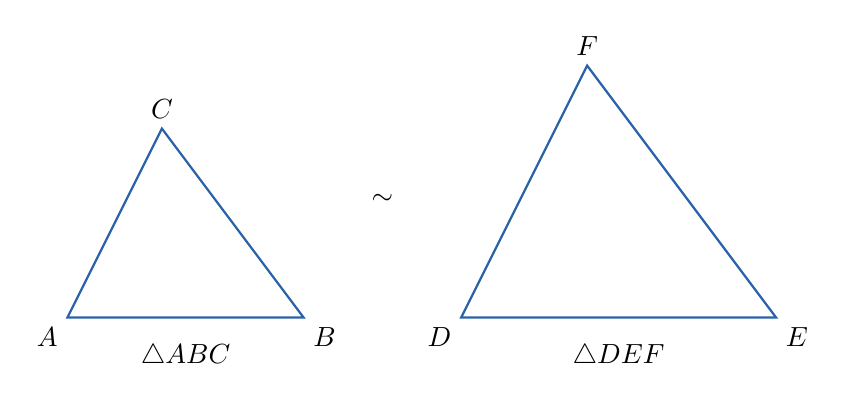
\begin{tikzpicture}
  % 左边三角形
  \coordinate (A) at (0,0);
  \coordinate (B) at (3,0);
  \coordinate (C) at (1.2,2.4);
  \draw[thick,mainblue] (A)--(B)--(C)--cycle;
  \node[below left] at (A) {$A$};
  \node[below right] at (B) {$B$};
  \node[above] at (C) {$C$};
  \node at (1.5,-0.5) {$\triangle ABC$};
  % 右边三角形
  \coordinate (D) at (5,0);
  \coordinate (E) at (9,0);
  \coordinate (F) at (6.6,3.2);
  \draw[thick,mainblue] (D)--(E)--(F)--cycle;
  \node[below left] at (D) {$D$};
  \node[below right] at (E) {$E$};
  \node[above] at (F) {$F$};
  \node at (7,-0.5) {$\triangle DEF$};
  % 相似符号
  \node at (4,1.5) {$\sim$};
\end{tikzpicture}
\end{center}

\textbf{相似比}：相似多边形对应边的比叫做\textbf{相似比}（或相似系数），记作 $k$。
若 $\triangle ABC\sim\triangle DEF$，相似比为 $k$，则
\[
\frac{AB}{DE}=\frac{BC}{EF}=\frac{AC}{DF}=k.
\]
\end{knowledgebox}

\begin{tipbox}[规律]
相似多边形具有以下性质：
\begin{enumerate}[nosep]
  \item 对应角相等；
  \item 对应边成比例；
  \item 周长之比等于相似比；
  \item 面积之比等于相似比的\textbf{平方}。
\end{enumerate}
\end{tipbox}

% ------- 27.3 相似三角形的判定 -------
\subsection*{27.3\quad 相似三角形的判定}

\begin{knowledgebox}[判定方法一：AA（两角对应相等）]
\textbf{两角对应相等，两三角形相似。}

即：在 $\triangle ABC$ 和 $\triangle DEF$ 中，若
\[
\angle A=\angle D,\quad \angle B=\angle E,
\]
则 $\triangle ABC\sim\triangle DEF$。

\medskip
\begin{center}
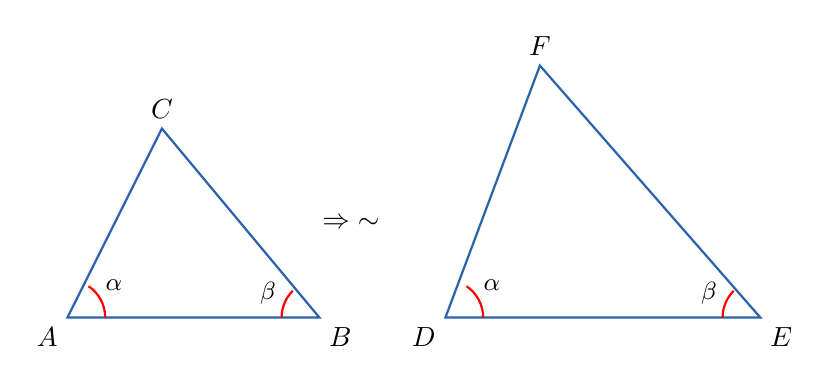
\begin{tikzpicture}[scale=0.8]
  \coordinate (A) at (0,0);
  \coordinate (B) at (4,0);
  \coordinate (C) at (1.5,3);
  \draw[thick,mainblue] (A)--(B)--(C)--cycle;
  \node[below left] at (A) {$A$};
  \node[below right] at (B) {$B$};
  \node[above] at (C) {$C$};
  \coordinate (D) at (6,0);
  \coordinate (E) at (11,0);
  \coordinate (F) at (7.5,4);
  \draw[thick,mainblue] (D)--(E)--(F)--cycle;
  \node[below left] at (D) {$D$};
  \node[below right] at (E) {$E$};
  \node[above] at (F) {$F$};
  % 标角
  \draw[red,thick] (A) ++(0.6,0) arc(0:56:0.6);
  \node at ($(A)+(35:0.9)$) {\small $\alpha$};
  \draw[red,thick] (B) ++(-0.6,0) arc(180:135:0.6);
  \node at ($(B)+(155:0.9)$) {\small $\beta$};
  \draw[red,thick] (D) ++(0.6,0) arc(0:56:0.6);
  \node at ($(D)+(35:0.9)$) {\small $\alpha$};
  \draw[red,thick] (E) ++(-0.6,0) arc(180:135:0.6);
  \node at ($(E)+(155:0.9)$) {\small $\beta$};
  \node at (4.5,1.5) {$\Rightarrow\;\sim$};
\end{tikzpicture}
\end{center}

这是最常用的判定方法。直角三角形中，只要有一个锐角相等，两直角三角形就相似。
\end{knowledgebox}

\begin{knowledgebox}[判定方法二：SAS（两边成比例且夹角相等）]
\textbf{两边对应成比例且夹角相等，两三角形相似。}

即：在 $\triangle ABC$ 和 $\triangle DEF$ 中，若
\[
\frac{AB}{DE}=\frac{AC}{DF},\quad \angle A=\angle D,
\]
则 $\triangle ABC\sim\triangle DEF$。

\medskip
\begin{center}
\begin{tikzpicture}[scale=0.8]
  \coordinate (A) at (0,0);
  \coordinate (B) at (4,0);
  \coordinate (C) at (1,2.5);
  \draw[thick,mainblue] (A)--(B)--(C)--cycle;
  \node[below left] at (A) {$A$};
  \node[below right] at (B) {$B$};
  \node[above] at (C) {$C$};
  \node at (2,-0.5) {\small $AB$};
  \node at (0.2,1.4) {\small $AC$};
  \draw[red,thick] (A) ++(0.6,0) arc(0:68:0.6);
  \\node at ($(A)+(\1)$) {\small $\alpha$};
  \coordinate (D) at (6,0);
  \coordinate (E) at (11,0);
  \coordinate (F) at (7.2,4);
  \draw[thick,mainblue] (D)--(E)--(F)--cycle;
  \node[below left] at (D) {$D$};
  \node[below right] at (E) {$E$};
  \node[above] at (F) {$F$};
  \node at (8.5,-0.5) {\small $DE$};
  \node at (6.3,2.2) {\small $DF$};
  \draw[red,thick] (D) ++(0.6,0) arc(0:68:0.6);
  \node at ($(D)+(38:0.85)$) {\small $\alpha$};
  \node at (5,1.5) {$\Rightarrow\;\sim$};
\end{tikzpicture}
\end{center}

\end{knowledgebox}

\begin{knowledgebox}[判定方法三：SSS（三边对应成比例）]
\textbf{三边对应成比例，两三角形相似。}

即：在 $\triangle ABC$ 和 $\triangle DEF$ 中，若
\[
\frac{AB}{DE}=\frac{BC}{EF}=\frac{AC}{DF},
\]
则 $\triangle ABC\sim\triangle DEF$。
\end{knowledgebox}

\begin{warnbox}[易错提醒]
\begin{enumerate}[nosep]
  \item SAS 判定中，夹角必须是成比例的两边\textbf{所夹的角}，不能是其他角。
  \item "两边对应成比例且其中一边的对角相等"\textbf{不能}判定相似（SSA 不能判定全等，也不能判定相似）。
  \item 直角三角形中，若斜边和一条直角边对应成比例，则两直角三角形相似（HL 相似）。
\end{enumerate}
\end{warnbox}

% ------- 27.4 相似三角形的性质 -------
\subsection*{27.4\quad 相似三角形的性质}

\begin{knowledgebox}[相似三角形的性质]
若 $\triangle ABC\sim\triangle DEF$，相似比为 $k$，则：
\begin{enumerate}[nosep]
  \item \textbf{对应角相等}：$\angle A=\angle D,\;\angle B=\angle E,\;\angle C=\angle F$；
  \item \textbf{对应边成比例}：$\dfrac{AB}{DE}=\dfrac{BC}{EF}=\dfrac{AC}{DF}=k$；
  \item \textbf{周长比}等于相似比：$\dfrac{C_{\triangle ABC}}{C_{\triangle DEF}}=k$；
  \item \textbf{面积比}等于相似比的平方：$\dfrac{S_{\triangle ABC}}{S_{\triangle DEF}}=k^2$；
  \item \textbf{对应线段之比}等于相似比：对应高之比、对应中线之比、对应角平分线之比都等于 $k$。
\end{enumerate}
\end{knowledgebox}

\begin{tipbox}[规律总结]
\begin{center}
\begin{tabular}{|c|c|}
\hline
\textbf{项目} & \textbf{与相似比 $k$ 的关系} \\
\hline
对应边 & $k$ \\
\hline
对应角 & 相等 \\
\hline
周长 & $k$ \\
\hline
对应高、中线、角平分线 & $k$ \\
\hline
面积 & $k^2$ \\
\hline
\end{tabular}
\end{center}
\end{tipbox}

% ------- 27.5 相似三角形的应用 -------
\subsection*{27.5\quad 相似三角形的应用与位似变换}

\begin{knowledgebox}[利用相似测高、测距]
利用相似三角形原理，可以在实际中测量不可直接度量的高度或距离。关键是构造两个相似三角形，利用对应边成比例列方程求解。

\medskip
\begin{center}
\begin{tikzpicture}[scale=0.7]
  % 地面
  \fill[lightgray!30] (-0.5,0) rectangle (10,-0.3);
  \draw[thick] (-0.5,0)--(10,0);
  % 物体（旗杆）
  \draw[very thick,mainblue] (7,0)--(7,6);
  \node[right] at (7,3) {\small 物体高 $h$};
  % 标杆
  \draw[very thick,red] (2,0)--(2,1.5);
  \node[left] at (2,0.75) {\small 标杆高 $a$};
  % 观测者眼睛
  \filldraw (0,0) circle(2pt) node[below] {\small 观测点};
  % 视线
  \draw[dashed,orange] (0,0)--(7,6);
  \draw[dashed,orange] (0,0)--(2,1.5);
  % 标注距离
  \draw[<->] (0,-0.4)--(2,-0.4);
  \node at (1,-0.7) {\small $d_1$};
  \draw[<->] (0,-0.4)--(7,-0.4);
  \node at (3.5,-0.7) {\small $d_2$};
\end{tikzpicture}
\end{center}

由相似关系：$\dfrac{h}{a}=\dfrac{d_2}{d_1}$，可得 $h=\dfrac{a\cdot d_2}{d_1}$。
\end{knowledgebox}

\begin{knowledgebox}[位似变换]
\textbf{位似}：如果两个图形不仅相似，而且对应顶点的连线相交于一点，对应边互相平行（或在同一条直线上），那么这两个图形叫做\textbf{位似图形}，这个交点叫做\textbf{位似中心}。

\medskip
\textbf{位似的性质：}
\begin{enumerate}[nosep]
  \item 位似图形一定是相似图形，相似比等于位似中心到对应顶点的距离之比。
  \item 位似图形上任意一对对应点到位似中心的距离之比等于相似比。
  \item 以位似中心为端点，过对应点的射线共线。
\end{enumerate}

\medskip
\begin{center}
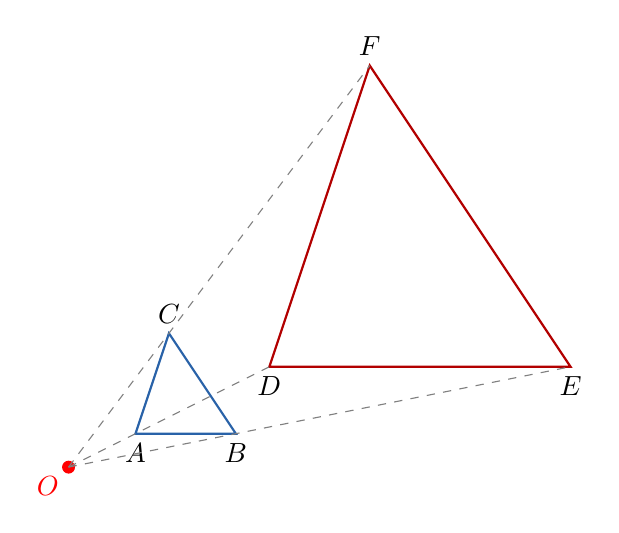
\begin{tikzpicture}[scale=0.85]
  % 位似中心
  \filldraw[red] (0,0) circle(2.5pt) node[below left] {$O$};
  % 小三角形
  \coordinate (A) at (1,0.5);
  \coordinate (B) at (2.5,0.5);
  \coordinate (C) at (1.5,2);
  \draw[thick,mainblue] (A)--(B)--(C)--cycle;
  \node[below] at (A) {$A$};
  \node[below] at (B) {$B$};
  \node[above] at (C) {$C$};
  % 大三角形
  \coordinate (D) at (3,1.5);
  \coordinate (E) at (7.5,1.5);
  \coordinate (F) at (4.5,6);
  \draw[thick,red!70!black] (D)--(E)--(F)--cycle;
  \node[below] at (D) {$D$};
  \node[below] at (E) {$E$};
  \node[above] at (F) {$F$};
  % 连线
  \draw[dashed,gray] (0,0)--(D);
  \draw[dashed,gray] (0,0)--(E);
  \draw[dashed,gray] (0,0)--(F);
\end{tikzpicture}
\end{center}
\end{knowledgebox}

% ============================================================
%  第二部分：例题精讲
% ============================================================
\section*{\textcolor{examorange}{二、例题精讲}}

\begin{examplebox}[【例题1】比例的基本性质]
已知 $\dfrac{x}{3}=\dfrac{y}{5}=\dfrac{z}{7}\neq0$，求 $\dfrac{x+y+z}{y}$ 的值。
\end{examplebox}

\textbf{解：}设 $\dfrac{x}{3}=\dfrac{y}{5}=\dfrac{z}{7}=k$（$k\neq0$），则
\[
x=3k,\quad y=5k,\quad z=7k.
\]
所以
\[
\frac{x+y+z}{y}=\frac{3k+5k+7k}{5k}=\frac{15k}{5k}=\boxed{3}.
\]

\begin{tipbox}[方法总结]
遇到连等式 $\dfrac{a}{m}=\dfrac{b}{n}=\dfrac{c}{p}$，常用"设 $k$ 法"，令比值为 $k$，将 $a,\,b,\,c$ 都用 $k$ 表示。
\end{tipbox}

\begin{examplebox}[【例题2】AA 判定相似]
如图，$\triangle ABC$ 中，$D$ 是 $AB$ 上一点，$E$ 是 $AC$ 上一点，$\angle ADE=\angle B$。求证：$\triangle ADE\sim\triangle ABC$。

\medskip
\begin{center}
\begin{tikzpicture}[scale=1]
  \coordinate (A) at (0,3);
  \coordinate (B) at (-2,0);
  \coordinate (C) at (4,0);
  \coordinate (D) at (-0.8,1.8);
  \coordinate (E) at (1.6,1.8);
  \draw[thick,mainblue] (A)--(B)--(C)--cycle;
  \draw[thick,red] (D)--(E);
  \node[above] at (A) {$A$};
  \node[below left] at (B) {$B$};
  \node[below right] at (C) {$C$};
  \node[left] at (D) {$D$};
  \node[right] at (E) {$E$};
  % 标角
  \draw[orange,thick] (A) ++(-0.5,-0.15) arc(-165:-130:0.5);
  \\node at ($(A)+(\1)$) {\small $\alpha$};
  \draw[orange,thick] (D) ++(0.4,0.1) arc(10:60:0.4);
  \node at ($(D)+(40:0.7)$) {\small $\alpha$};
\end{tikzpicture}
\end{center}
\end{examplebox}

\textbf{证明：}
\begin{itemize}[nosep]
  \item 在 $\triangle ADE$ 和 $\triangle ABC$ 中：
  \item $\angle A=\angle A$（公共角）；
  \item $\angle ADE=\angle B$（已知）；
  \item 由"两角对应相等，两三角形相似"（AA），得 $\triangle ADE\sim\triangle ABC$。\qed
\end{itemize}

\begin{examplebox}[【例题3】SAS 判定相似]
如图，在 $\triangle ABC$ 中，$D$、$E$ 分别是 $AB$、$AC$ 上的点，$AD=2$，$DB=4$，$AE=3$，$EC=6$。求证：$\triangle ADE\sim\triangle ABC$。

\medskip
\begin{center}
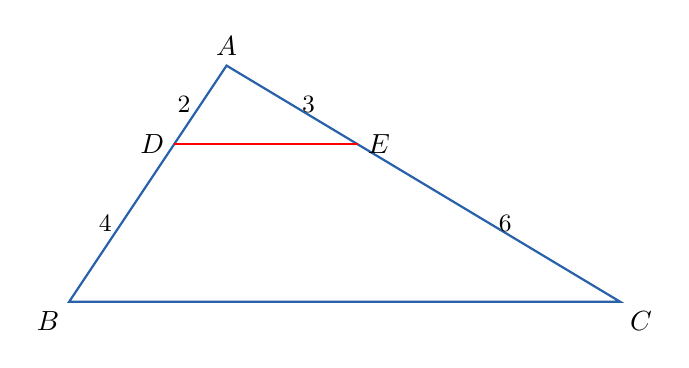
\begin{tikzpicture}[scale=1]
  \coordinate (A) at (0,3);
  \coordinate (B) at (-2,0);
  \coordinate (C) at (5,0);
  \coordinate (D) at (-0.67,2);
  \coordinate (E) at (1.67,2);
  \draw[thick,mainblue] (A)--(B)--(C)--cycle;
  \draw[thick,red] (D)--(E);
  \node[above] at (A) {$A$};
  \node[below left] at (B) {$B$};
  \node[below right] at (C) {$C$};
  \node[left] at (D) {$D$};
  \node[right] at (E) {$E$};
  \node[left] at ($(A)!0.5!(D)$) {\small $2$};
  \node[left] at ($(D)!0.5!(B)$) {\small $4$};
  \node[right] at ($(A)!0.5!(E)$) {\small $3$};
  \node[right] at ($(E)!0.5!(C)$) {\small $6$};
\end{tikzpicture}
\end{center}
\end{examplebox}

\textbf{证明：}
\begin{itemize}[nosep]
  \item $AB=AD+DB=2+4=6$，$AC=AE+EC=3+6=9$。
  \item $\dfrac{AD}{AB}=\dfrac{2}{6}=\dfrac{1}{3}$，$\dfrac{AE}{AC}=\dfrac{3}{9}=\dfrac{1}{3}$。
  \item 所以 $\dfrac{AD}{AB}=\dfrac{AE}{AC}$，且 $\angle A=\angle A$（公共角）。
  \item 由 SAS 判定，$\triangle ADE\sim\triangle ABC$。\qed
\end{itemize}

\begin{examplebox}[【例题4】相似三角形性质——面积比]
如图，$\triangle ABC\sim\triangle DEF$，$AB=6$，$DE=9$，$\triangle ABC$ 的面积为 $8$，求 $\triangle DEF$ 的面积。
\end{examplebox}

\textbf{解：}相似比为
\[
k=\frac{AB}{DE}=\frac{6}{9}=\frac{2}{3}.
\]
由面积比等于相似比的平方，得
\[
\frac{S_{\triangle ABC}}{S_{\triangle DEF}}=k^2=\left(\frac{2}{3}\right)^2=\frac{4}{9}.
\]
因此
\[
S_{\triangle DEF}=\frac{9}{4}\times S_{\triangle ABC}=\frac{9}{4}\times 8=\boxed{18}.
\]

\begin{examplebox}[【例题5】证明题——平行线与相似]
如图，在 $\triangle ABC$ 中，$DE\parallel BC$，$D$ 在 $AB$ 上，$E$ 在 $AC$ 上。$AD=4$，$DB=2$，$BC=9$。求 $DE$ 的长。

\medskip
\begin{center}
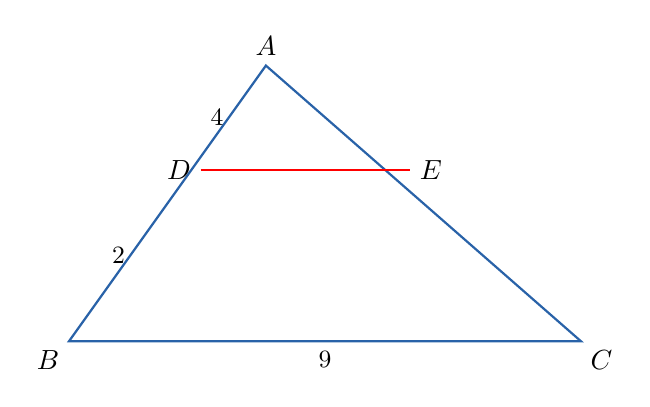
\begin{tikzpicture}[scale=1]
  \coordinate (A) at (0,3.5);
  \coordinate (B) at (-2.5,0);
  \coordinate (C) at (4,0);
  \coordinate (D) at (-0.83,2.17);
  \coordinate (E) at (1.83,2.17);
  \draw[thick,mainblue] (A)--(B)--(C)--cycle;
  \draw[thick,red] (D)--(E);
  \node[above] at (A) {$A$};
  \node[below left] at (B) {$B$};
  \node[below right] at (C) {$C$};
  \node[left] at (D) {$D$};
  \node[right] at (E) {$E$};
  \node[left] at ($(A)!0.5!(D)$) {\small $4$};
  \node[left] at ($(D)!0.5!(B)$) {\small $2$};
  \node[below] at ($(B)!0.5!(C)$) {\small $9$};
\end{tikzpicture}
\end{center}
\end{examplebox}

\textbf{解：}
\begin{itemize}[nosep]
  \item 因为 $DE\parallel BC$，所以 $\angle ADE=\angle B$，$\angle AED=\angle C$（同位角）。
  \item 又 $\angle A=\angle A$（公共角），由 AA 得 $\triangle ADE\sim\triangle ABC$。
  \item 相似比为 $\dfrac{AD}{AB}=\dfrac{4}{4+2}=\dfrac{2}{3}$。
  \item 所以 $\dfrac{DE}{BC}=\dfrac{2}{3}$，即 $\dfrac{DE}{9}=\dfrac{2}{3}$。
  \item 解得 $DE=\boxed{6}$。
\end{itemize}

\begin{tipbox}[重要结论]
\textbf{平行于三角形一边的直线截另外两边（或其延长线），所得三角形与原三角形相似。}
这是 AA 判定的一个典型应用，非常常用。
\end{tipbox}

\begin{examplebox}[【例题6】综合证明——相似与线段比]
如图，$\triangle ABC$ 中，$\angle BAC=90°$，$AD\perp BC$ 于 $D$。

(1) 求证：$\triangle ABD\sim\triangle CBA\sim\triangle CAD$；

(2) 若 $BD=4$，$DC=9$，求 $AD$ 的长。

\medskip
\begin{center}
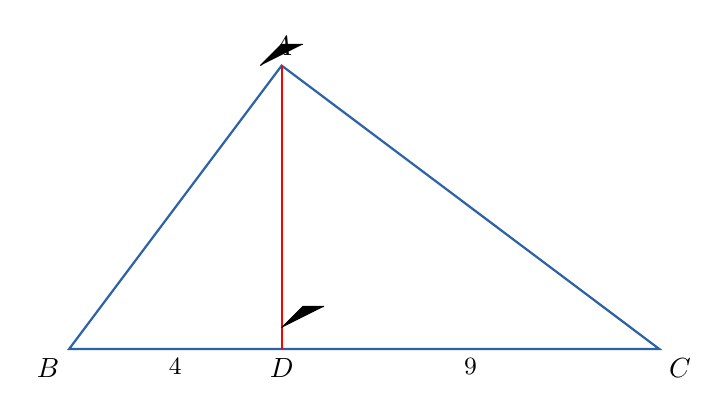
\begin{tikzpicture}[scale=0.9]
  \coordinate (A) at (0,4);
  \coordinate (B) at (-3,0);
  \coordinate (C) at (5.33,0);
  \coordinate (D) at (0,0);
  \draw[thick,mainblue] (A)--(B)--(C)--cycle;
  \draw[thick,red] (A)--(D);
  \filldraw (A) ++(-0.3,0) -- ++(0.3,0.3) -- ++(0.3,0);
  \filldraw (D) ++(0,0.3) -- ++(0.3,0.3) -- ++(0.3,0);
  \node[above] at (A) {$A$};
  \node[below left] at (B) {$B$};
  \node[below right] at (C) {$C$};
  \node[below] at (D) {$D$};
  \node[below] at ($(B)!0.5!(D)$) {\small $4$};
  \node[below] at ($(D)!0.5!(C)$) {\small $9$};
\end{tikzpicture}
\end{center}
\end{examplebox}

\textbf{解：}

(1) \textbf{证明 $\triangle ABD\sim\triangle CBA$：}

在 $\triangle ABD$ 和 $\triangle CBA$ 中：
\begin{itemize}[nosep]
  \item $\angle B=\angle B$（公共角）；
  \item $\angle BDA=\angle BAC=90°$；
  \item 由 AA，$\triangle ABD\sim\triangle CBA$。
\end{itemize}

\textbf{证明 $\triangle CAD\sim\triangle CBA$：}

在 $\triangle CAD$ 和 $\triangle CBA$ 中：
\begin{itemize}[nosep]
  \item $\angle C=\angle C$（公共角）；
  \item $\angle CDA=\angle CAB=90°$；
  \item 由 AA，$\triangle CAD\sim\triangle CBA$。
\end{itemize}

由传递性，$\triangle ABD\sim\triangle CAD\sim\triangle CBA$。\qed

\medskip
(2) 由 $\triangle ABD\sim\triangle CAD$，对应边成比例：
\[
\frac{BD}{AD}=\frac{AD}{CD}.
\]
即 $AD^2=BD\times CD=4\times9=36$，所以 $AD=\boxed{6}$。

\begin{tipbox}[射影定理]
直角三角形中，斜边上的高将直角三角形分成两个与原三角形相似的小三角形。由此可得：
\[
AD^2=BD\cdot DC,\quad AB^2=BD\cdot BC,\quad AC^2=CD\cdot BC.
\]
这就是\textbf{射影定理}（也叫"投影定理"），是相似三角形的经典应用。
\end{tipbox}

% ============================================================
%  第三部分：应用题
% ============================================================
\section*{\textcolor{apppurple}{三、应用题}}

\begin{appbox}[【应用1】利用影长测高]
小明想测量学校旗杆的高度。他在地面上竖一根 $2\,\text{m}$ 长的标杆，测得标杆的影长为 $1.5\,\text{m}$，同时测得旗杆的影长为 $6\,\text{m}$。求旗杆的高度。（同一时刻阳光的入射角相同）

\medskip
\begin{center}
\begin{tikzpicture}[scale=0.6]
  \fill[lightgray!20] (-1,0) rectangle (12,-0.3);
  \draw[thick] (-1,0)--(12,0);
  % 旗杆
  \draw[very thick,mainblue] (8,0)--(8,8);
  \node[right] at (8,4) {\small 旗杆 $h$};
  % 标杆
  \draw[very thick,red] (2,0)--(2,2);
  \node[left] at (2,1) {\small $2\,$m};
  % 阳光
  \draw[dashed,orange] (8,8)--(10.5,0);
  \draw[dashed,orange] (2,2)--(3.5,0);
  % 影长
  \draw[<->] (8,-0.6)--(10.5,-0.6);
  \node at (9.25,-0.9) {\small $6\,$m};
  \draw[<->] (2,-0.6)--(3.5,-0.6);
  \node at (2.75,-0.9) {\small $1.5\,$m};
\end{tikzpicture}
\end{center}
\end{appbox}

\textbf{解：}同一时刻阳光入射角相同，因此物体和影长构成的直角三角形相似。

设旗杆高为 $h$，则
\[
\frac{h}{6}=\frac{2}{1.5},
\]
解得 $h=\dfrac{6\times2}{1.5}=\boxed{8}\,\text{m}$。

\begin{appbox}[【应用2】利用相似测河宽]
如图，为测量河宽 $AB$，在河对岸选定目标 $C$，在此岸取 $D$、$E$ 两点，使 $A$、$D$、$E$ 在同一直线上。再在 $DE$ 上取 $F$ 点，使 $CF\perp DE$。测得 $AD=10\,\text{m}$，$DE=40\,\text{m}$，$EF=20\,\text{m}$，$CF=30\,\text{m}$。求河宽 $AB$。

\medskip
\begin{center}
\begin{tikzpicture}[scale=0.5]
  % 河
  \fill[blue!10] (-1,-1) rectangle (12,3);
  \draw[blue,thick] (-1,3)--(12,3);
  \draw[blue,thick] (-1,-1)--(12,-1);
  \node at (5.5,1) {\small 河};
  % 点
  \coordinate (A) at (0,3);
  \coordinate (D) at (2,3);
  \coordinate (E) at (10,3);
  \coordinate (B) at (0,-1);
  \coordinate (C) at (10,-1);
  \coordinate (F) at (10,3);
  \filldraw (A) circle(2pt) node[above] {$A$};
  \filldraw (D) circle(2pt) node[above] {$D$};
  \filldraw (E) circle(2pt) node[above] {$E$};
  \filldraw (B) circle(2pt) node[below] {$B$};
  \filldraw (C) circle(2pt) node[below] {$C$};
  \filldraw (F) circle(2pt) node[above right] {$F$};
  % 线段
  \draw[thick,mainblue] (B)--(C);
  \draw[thick,red] (A)--(C);
  \draw[thick,red] (D)--(C);
  \draw[thick] (C)--(F);
  % 标注
  \node[above] at ($(A)!0.5!(D)$) {\small $10$};
  \node[above] at ($(D)!0.5!(E)$) {\small $40$};
  \node[right] at ($(E)!0.5!(C)$) {\small $20$};
  \node at (11.5,1) {\small $CF=30$};
\end{tikzpicture}
\end{center}
\end{appbox}

\textbf{解：}
\begin{itemize}[nosep]
  \item $\angle ADB=\angle EDF=90°$（$A$、$D$、$E$ 共线，$AB\perp DE$），$\angle ABD=\angle EFC=90°$。
  \item 实际上，由 $\angle BAC=\angle CEF$（$AB\parallel CF$ 同垂直于河岸，同位角），$\angle ABD=\angle EFC=90°$。
  \item 由 AA，$\triangle ABD\sim\triangle EFC$。
  \item $\dfrac{AB}{EF}=\dfrac{AD}{FC}$，即 $\dfrac{AB}{20}=\dfrac{10}{30}$。
  \item 解得 $AB=\dfrac{20\times10}{30}=\boxed{\dfrac{20}{3}}\approx6.67\,\text{m}$。
\end{itemize}

\begin{appbox}[【应用3】位似缩放——地图比例尺]
某小区的平面示意图按 $1:500$ 的比例尺绘制。在图上量得小区长为 $12\,\text{cm}$，宽为 $8\,\text{cm}$。
\begin{enumerate}[nosep]
  \item 求小区实际的长和宽；
  \item 求小区的实际面积；
  \item 图上面积与实际面积的比是多少？
\end{enumerate}
\end{appbox}

\textbf{解：}
\begin{enumerate}
  \item 相似比（图:实际）$=1:500$。
  \begin{itemize}[nosep]
    \item 实际长 $=12\times500=6000\,\text{cm}=60\,\text{m}$。
    \item 实际宽 $=8\times500=4000\,\text{cm}=40\,\text{m}$。
  \end{itemize}
  \item 实际面积 $=60\times40=\boxed{2400}\,\text{m}^2$。
  \item 面积比 $=$ 相似比的平方 $=\left(\dfrac{1}{500}\right)^2=\dfrac{1}{250000}$。
\end{enumerate}

% ============================================================
%  第四部分：课堂练习
% ============================================================
\section*{\textcolor{tipgreen}{四、课堂练习}}

\begin{enumerate}
  \item 已知 $\dfrac{a}{2}=\dfrac{b}{3}=\dfrac{c}{4}$，求 $\dfrac{a+b}{b+c}$ 的值。

  \item 在 $\triangle ABC$ 和 $\triangle DEF$ 中，$\angle A=50°$，$\angle B=70°$，$\angle D=50°$，$\angle E=70°$。这两个三角形相似吗？为什么？

  \item $\triangle ABC\sim\triangle DEF$，相似比为 $3:5$。若 $\triangle ABC$ 的周长为 $36$，求 $\triangle DEF$ 的周长。

  \item 如图，在 $\triangle ABC$ 中，$DE\parallel BC$，$AD=3$，$AB=7$，$DE=5$，求 $BC$ 的长。

  \medskip
  \begin{center}
  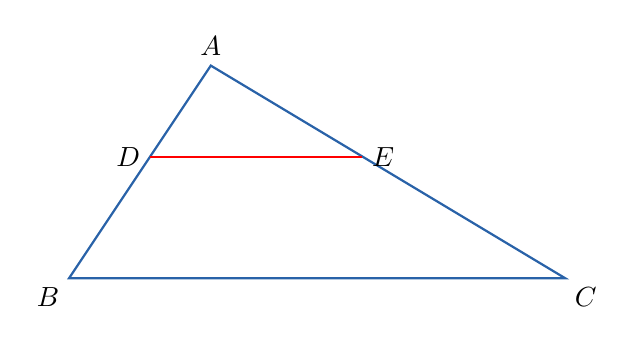
\begin{tikzpicture}[scale=0.9]
    \coordinate (A) at (0,3);
    \coordinate (B) at (-2,0);
    \coordinate (C) at (5,0);
    \coordinate (D) at (-0.86,1.71);
    \coordinate (E) at (2.14,1.71);
    \draw[thick,mainblue] (A)--(B)--(C)--cycle;
    \draw[thick,red] (D)--(E);
    \node[above] at (A) {$A$};
    \node[below left] at (B) {$B$};
    \node[below right] at (C) {$C$};
    \node[left] at (D) {$D$};
    \node[right] at (E) {$E$};
  \end{tikzpicture}
  \end{center}

  \item 两面平行的镜子之间有一棵小树。小树高 $1.6\,\text{m}$，在镜子中的像高 $2.4\,\text{m}$。如果镜子距小树 $3\,\text{m}$，求像到镜子的距离。

  \item $\triangle ABC$ 中，$\angle C=90°$，$CD\perp AB$ 于 $D$，$AC=6$，$BC=8$。求 $CD$ 的长。

  \item 如图，梯形 $ABCD$ 中，$AB\parallel CD$，对角线 $AC$、$BD$ 交于点 $O$。若 $AB=6$，$CD=4$，$S_{\triangle AOB}=9$，求 $S_{\triangle COD}$。

  \medskip
  \begin{center}
  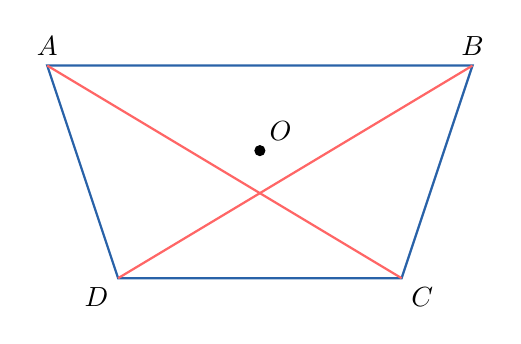
\begin{tikzpicture}[scale=0.9]
    \coordinate (A) at (0,3);
    \coordinate (B) at (6,3);
    \coordinate (C) at (5,0);
    \coordinate (D) at (1,0);
    \coordinate (O) at (3,1.8);
    \draw[thick,mainblue] (A)--(B)--(C)--(D)--cycle;
    \draw[thick,red!60] (A)--(C);
    \draw[thick,red!60] (B)--(D);
    \filldraw (O) circle(2pt) node[above right] {$O$};
    \node[above] at (A) {$A$};
    \node[above] at (B) {$B$};
    \node[below right] at (C) {$C$};
    \node[below left] at (D) {$D$};
  \end{tikzpicture}
  \end{center}

  \item 如图，$\triangle ABC$ 中，$D$ 是 $BC$ 上一点，$\angle BAD=\angle C$。若 $BD=3$，$DC=5$，$AC=10$，求 $AB$ 的长。

  \medskip
  \begin{center}
  \begin{tikzpicture}[scale=1]
    \coordinate (A) at (0,4);
    \coordinate (B) at (-3,0);
    \coordinate (C) at (5,0);
    \coordinate (D) at (0,0);
    \draw[thick,mainblue] (A)--(B)--(C)--cycle;
    \draw[thick,red] (A)--(D);
    \node[above] at (A) {$A$};
    \node[below left] at (B) {$B$};
    \node[below right] at (C) {$C$};
    \node[below] at (D) {$D$};
    \node[below] at ($(B)!0.5!(D)$) {\small $3$};
    \node[below] at ($(D)!0.5!(C)$) {\small $5$};
  \end{tikzpicture}
  \end{center}
\end{enumerate}

\begin{knowledgebox}[参考答案]
\begin{enumerate}
  \item 设 $\dfrac{a}{2}=\dfrac{b}{3}=\dfrac{c}{4}=k$，则 $a=2k,\,b=3k,\,c=4k$。
  \[
  \frac{a+b}{b+c}=\frac{2k+3k}{3k+4k}=\frac{5k}{7k}=\boxed{\dfrac{5}{7}}.
  \]

  \item 相似。$\angle A=\angle D=50°$，$\angle B=\angle E=70°$，由 AA 判定，$\triangle ABC\sim\triangle DEF$。

  \item 相似比为 $k=3:5$，周长比也为 $3:5$。
  \[
  \frac{36}{C_{\triangle DEF}}=\frac{3}{5}\;\Rightarrow\;C_{\triangle DEF}=\frac{36\times5}{3}=\boxed{60}.
  \]

  \item $DE\parallel BC\;\Rightarrow\;\triangle ADE\sim\triangle ABC$，相似比 $=\dfrac{AD}{AB}=\dfrac{3}{7}$。
  \[
  \frac{DE}{BC}=\frac{3}{7}\;\Rightarrow\;\frac{5}{BC}=\frac{3}{7}\;\Rightarrow\;BC=\boxed{\dfrac{35}{3}}.
  \]

  \item 利用相似：$\dfrac{\text{像高}}{\text{物高}}=\dfrac{\text{像到镜面距离}}{\text{物到镜面距离}}$，即 $\dfrac{2.4}{1.6}=\dfrac{d}{3}$，解得 $d=\boxed{4.5}\,\text{m}$。

  \item 由勾股定理，$AB=\sqrt{AC^2+BC^2}=\sqrt{36+64}=10$。由面积法：
  \[
  S_{\triangle ABC}=\frac{1}{2}\times AC\times BC=\frac{1}{2}\times6\times8=24,
  \]
  又 $S_{\triangle ABC}=\frac{1}{2}\times AB\times CD$，所以 $\frac{1}{2}\times10\times CD=24$，$CD=\boxed{4.8}$。

  \item $AB\parallel CD\;\Rightarrow\;\triangle AOB\sim\triangle COD$，相似比 $=\dfrac{AB}{CD}=\dfrac{6}{4}=\dfrac{3}{2}$。
  \[
  \frac{S_{\triangle AOB}}{S_{\triangle COD}}=\left(\frac{3}{2}\right)^2=\frac{9}{4}.
  \]
  $S_{\triangle COD}=\dfrac{4}{9}\times9=\boxed{4}$。

  \item $\angle BAD=\angle C$，$\angle B=\angle B$（公共角），由 AA 得 $\triangle ABD\sim\triangle CBA$。
  \[
  \frac{AB}{BC}=\frac{BD}{AB}\;\Rightarrow\;AB^2=BD\times BC=3\times(3+5)=24.
  \]
  $AB=\sqrt{24}=\boxed{2\sqrt{6}}$。
\end{enumerate}
\end{knowledgebox}

\vfill
\begin{center}
\small\textcolor{gray}{本讲义仅供教学参考，例题可根据学生水平调整难度。}
\end{center}

\end{document}
